\documentclass{article}
\usepackage[T1]{fontenc}
\usepackage{lmodern}
\usepackage{graphicx}
\usepackage{amsmath,amssymb}
\usepackage[a4paper,margin=2cm]{geometry}
\usepackage[absolute,overlay]{textpos}
\setlength{\TPHorizModule}{1mm}
\setlength{\TPVertModule}{1mm}
\usepackage[indonesian]{babel}
\usepackage{hyperref}
\setlength{\emergencystretch}{2em}
% unit: Halaman 35

\begin{document}

% === Halaman 35 (llm) ===

\vspace{210.87mm}

Demo kallkulator ECC online: \url{https://andrea.corbellini.name/ecc/interactive/reals-add.html}

\vspace{10mm}

Point addition over the elliptic curve $y^2 = x^3 + 1x + 6$ in $\mathbb{F}_{11}$. The curve has 13 points (including the point at infinity).

% deskripsi: Screenshot kalkulator interaktif Elliptic Curve point addition (Fp) yang menampilkan grafik koordinat, input parameter kurva (a=1, b=6), field p=11, serta koordinat titik P, Q, dan hasil penjumlahan R=P+Q.
% bbox normalisasi: [0.0300, 0.1400, 0.9600, 0.8500]
\begin{textblock*}{195.30mm}(6.30mm,41.58mm)
\noindent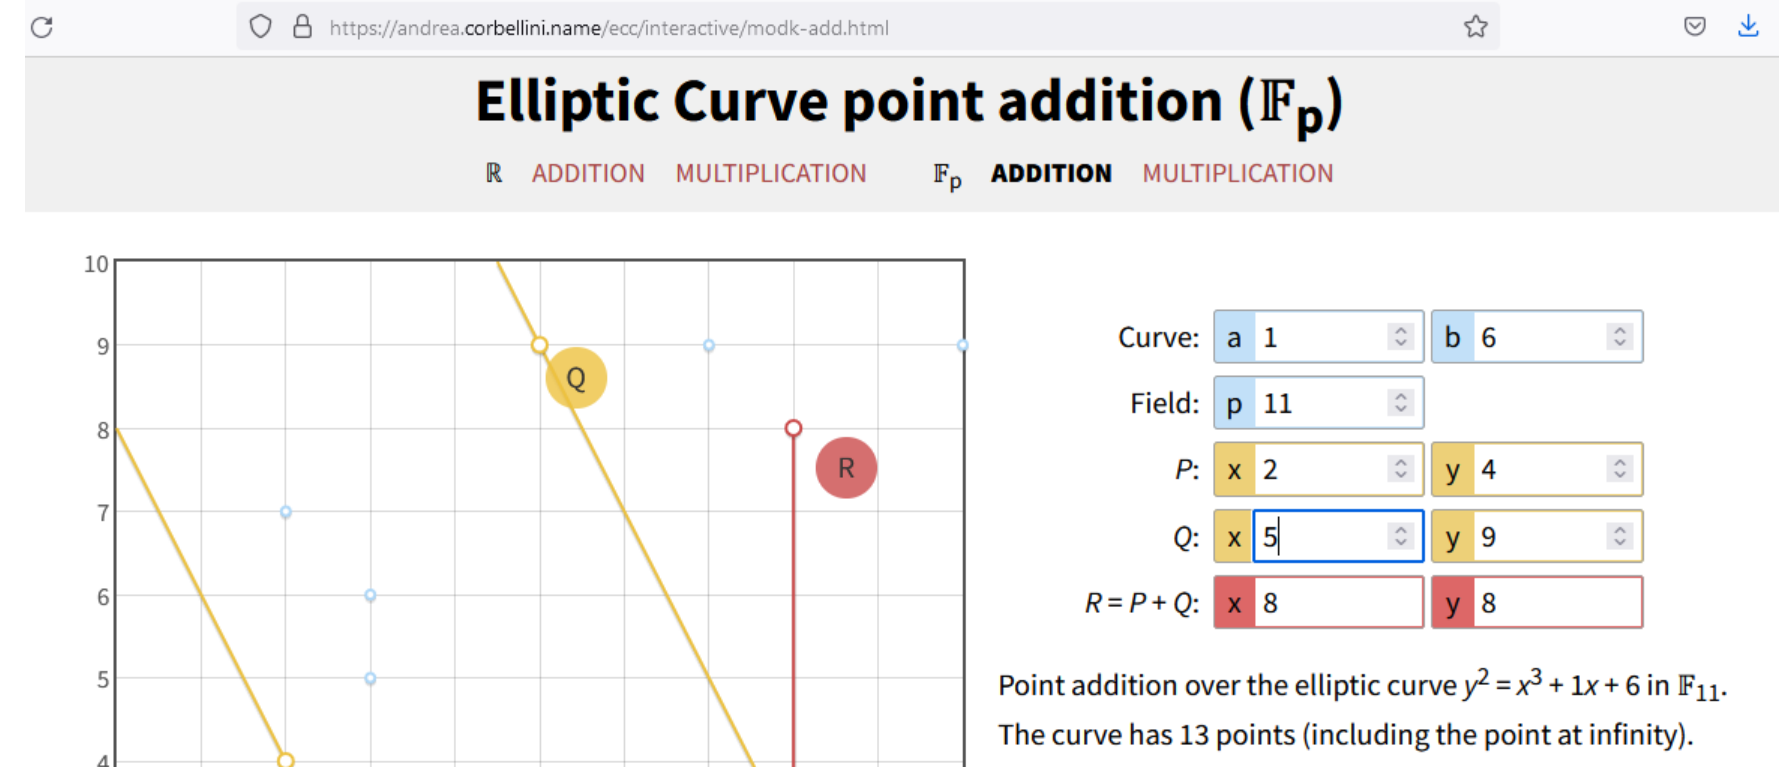
\includegraphics[width=195.30mm,height=210.87mm]{../../images/llm/page_035_img_01.png}%
\end{textblock*}

\end{document}
